% !TEX root =../dissertation.tex
\documentclass$[./dissertation.tex]${subfiles}
\begin{document}
\chapter{Training a Supervised Cilia Segmentation Model from Self-Supervision}



Cilia are organelles found on the surface of some cells in the human body that sweep rhythmically to transport substances. Dysfunctional cilia are indicative of diseases that can disrupt organs such as the lungs and kidneys. Understanding cilia behavior is essential in diagnosing and treating such diseases. But, the tasks of automatically analysing cilia are often a labor and time-intensive since there is a lack of automated segmentation. In this work we overcome this bottleneck by developing a robust, self-supervised framework exploiting the visual similarity of normal and dysfunctional cilia. This framework generates pseudolabels from optical flow motion vectors, which serve as training data for a semi-supervised neural network. Our approach eliminates the need for manual annotations, enabling accurate and efficient segmentation of both motile and immotile cilia.

\section{Introduction}

Cilia are hair-like membranes that extend out from the surface of the cells and are present on a variety of cell types such as lungs and brain ventricles and can be found in the majority of vertebrate cells. Categorized into motile and primary, motile cilia can help the cell to propel, move the flow of fluid, or fulfill sensory functions, while primary cilia act as signal receivers, translating extracellular signals into cellular responses $[@doi:10.1007/978-94-007-5808-7_1]$. Ciliopathies is the term commonly used to describe diseases caused by ciliary dysfunction. These disorders can result in serious issues such as blindness, neurodevelopmental defects, or obesity $[@Hansen2021-fd]$. Motile cilia beat in a coordinated manner with a specific frequency and pattern $[@doi:10.1016/j.compfluid.2011.05.016]$. Stationary, dyskinetic, or slow ciliary beating indicates ciliary defects. Ciliary beating is a fundamental biological process that is essential for the proper functioning of various organs, which makes understanding the ciliary phenotypes a crucial step towards understanding ciliopathies and the conditions stemming from it $[@zain2022low]$.

Identifying and categorizing the motion of cilia is an essential step towards understanding ciliopathies. However, this is generally an expert-intensive process. Studies have proposed methods that automate the ciliary motion assessment $[@zain2020towards]$. These methods rely on large amounts of labeled data that are annotated manually which is a costly, time-consuming, and error-prone task. Consequently, a significant bottleneck to automating cilia analysis is a lack of automated segmentation. Segmentation has remained a bottleneck of the pipeline due to the poor performance of even state-of-the-art models on some datasets. These datasets tend to exhibit significant spatial artifacts (light diffraction, out-of-focus cells, etc.) which confuse traditional image segmentation models $[@doi:10.48550/arXiv.1803.07534]$.

Video segmentation techniques tend to be more robust to such noise, but still struggle due to the wild inconsistencies in cilia behavior: while healthy cilia have regular and predictable movements, unhealthy cilia display a wide range of motion, including a lack of motion altogether $[@doi:10.1002/ppul.24078]$. This lack of motion especially confounds movement-based methods which otherwise have no way of discerning the cilia from other non-cilia parts of the video. Both image and video segmentation techniques tend to require expert-labeled ground truth segmentation masks. Image segmentation requires the masks in order to effectively train neural segmentation models to recognize cilia, rather than other spurious textures. Video segmentation, by contrast, requires these masks in order to properly recognize both healthy and diseased cilia as a single cilia category, especially when the cilia show no movement.

To address this challenge, we propose a two-stage image segmentation model designed to obviate the need for expert-drawn masks. We first build a corpus of segmentation masks based on optical flow (OF) thresholding over a subset of healthy training data with guaranteed motility. We then train a semi-supervised neural segmentation model to identify both motile and immotile data as a single segmentation category, using the flow-generated masks as “pseudolabels”. These pseudolabels operate as “ground truth” for the model while acknowledging the intrinsic uncertainty of the labels. The fact that motile and immotile cilia tend to be visually similar in snapshot allows us to generalize the domain of the model from motile cilia to all cilia. Combining these stages results in a semi-supervised framework that does not rely on any expert-drawn ground-truth segmentation masks, paving the way for full automation of a general cilia analysis pipeline.
% The rest of this article is structured as follows: The Background section enumerates the studies relevant to our methodology, followed by a detailed description of our approach in the Methodology section. Finally, the next section delineates our experiment and provides a discussion of the results obtained.
\section{Background}
Dysfunction in ciliary motion indicates diseases known as ciliopathies, which can disrupt the functionality of critical organs like the lungs and kidneys. Understanding ciliary motion is crucial for diagnosing and understanding these conditions. The development of diagnosis and treatment requires the measurement of different cell properties including size, shape, and motility $[@vaezi2022novel]$.

Accurate analysis of ciliary motion is essential but challenging due to the limitations of manual analysis, which is /labor-intensive, subjective, and prone to error. $[@zain2020towards]$ proposed a modular generative pipeline that automates ciliary motion analysis by segmenting, representing, and modeling the dynamic behavior of cilia, thereby reducing the need for expert intervention and improving diagnostic consistency. $[@quinn2015automated]$ developed a computational pipeline using dynamic texture analysis and machine learning to objectively and quantitatively assess ciliary motion, achieving over 90\% classification accuracy in identifying abnormal ciliary motion associated with diseases like primary ciliary dyskinesia (PCD). Additionally, $[@zain2022low]$ explored advanced feature extraction techniques like Zero-phase PCA Sphering (ZCA) and Sparse Autoencoders (SAE) to enhance cilia segmentation accuracy. These methods address challenges posed by noisy, partially occluded, and out-of-phase imagery, ultimately improving the overall performance of ciliary motion analysis pipelines. Collectively, these approaches aim to enhance diagnostic accuracy and efficiency, making ciliary motion analysis more accessible and reliable, thereby improving patient outcomes through early and accurate detection of ciliopathies. However, these studies rely on manually labeled data. The segmentation masks and ground-truth annotations, which are essential for training the models and validating their performance, are generated by expert reviewers. This dependence on manually labeled data is a significant limitation making automated cilia segmentation the bottleneck to automating cilia analysis.

In the biomedical field, where labeled data is often scarce and costly to obtain, several solutions have been proposed to augment and utilize available data effectively. These include semi-supervised learning $[@YAKIMOVICH2021100383]$, $[@van2020survey]$, which utilizes both labeled and unlabeled data to enhance learning accuracy by leveraging the data’s underlying distribution. Active learning $[@settles2009active]$ focuses on selectively querying the most informative data points for expert labeling, optimizing the training process by using the most valuable examples. Data augmentation techniques $[@10.3389/fcvm.2020.00105]$, $[@Krois2021]$, $[@10.1148/ryai.2020190195]$, $[@Sandfort2019]$, $[@YAKIMOVICH2021100383]$, $[@van2001art]$, $[@krizhevsky2012imagenet]$, $[@ronneberger2015u]$, such as image transformations and synthetic data generation through Generative Adversarial Networks $[@goodfellow2014generative]$, $[@yi2019generative]$, increase the diversity and volume of training data, enhancing model robustness and reducing overfitting. Transfer learning $[@YAKIMOVICH2021100383]$, $[@Sanford2020-yg]$, $[@NEURIPS2019_eb1e7832]$, $[@hutchinson2017overcoming]$ transfers knowledge from one task to another, minimizing the need for extensive labeled data in new tasks. Self-supervised learning $[@kim2019self]$, $[@kolesnikov2019revisiting]$, $[@mahendran2019cross]$ creates its labels by defining a pretext task, like predicting the position of a randomly cropped image patch, aiding in the learning of useful data representations. Additionally, few-shot, one-shot, and zero-shot learning techniques $[@li2006one]$, $[@miller2000learning]$ are designed to operate with minimal or no labeled examples, relying on generalization capabilities or metadata for making predictions about unseen classes.

A promising approach to overcome the dependency on manually labeled data is the use of unsupervised methods to generate ground truth masks. Unsupervised methods do not require prior knowledge of the data $[@khatibi2021proposing]$. Using domain-specific cues unsupervised learning techniques can automatically discover patterns and structures in the data without the need for labeled examples, potentially simplifying the process of generating accurate segmentation masks for cilia. Inspired by advances in unsupervised methods for image segmentation, in this work, we firstly compute the motion vectors using optical flow of the ciliary regions and then apply autoregressive modelling to capture their temporal dynamics. Autoregressive modelling is advantageous since the labels are features themselves. By analyzing the OF vectors, we can identify the characteristic motion of cilia, which allows us to generate pseudolabels as ground truth segmentation masks. These pseudolabels are then used to train a robust semi-supervised neural network, enabling accurate and automated segmentation of both motile and immotile cilia.


\section{Methodology}

Dynamic textures, such as sea waves, smoke, and foliage, are sequences of images of moving scenes that exhibit certain stationarity properties in time $[@doretto2003dynamic]$. Similarly, ciliary motion can be considered as dynamic textures for their orderly rhythmic beating. Taking advantage of this temporal regularity in ciliary motion, OF can be used to compute the flow vectors of each pixel of high-speed videos of cilia. In conjunction with OF, autoregressive (AR) parameterization of the OF property of the video yields a manifold that quantifies the characteristic motion in the cilia. The low dimension of this manifold contains the majority of variations within the data, which can then be used to segment the motile ciliary regions.
\section{Optical Flow Properties}
Taking advantage of this temporal regularity in ciliary motion, we use OF to capture the motion vectors of ciliary regions in high-speed videos. OF provides the horizontal u and vertical v components of the motion for each pixel. From these motion vectors, several components can be derived such as the magnitude, direction, divergence, and importantly, the curl (rotation). The curl, in this context, represents the rotational motion of the cilia, which is indicative of their rhythmic beating patterns. We extract flow vectors of the video recording of cilia, under the assumption that pixel intensity remains constant throughout the video.

\begin{equation}
	I(x,y,t)=I(x+u\delta t,y+v\delta t,t+\delta t)
	\label{eq:eq1}
\end{equation}


\eqref{eq:eq1} Where $I_{x,y,t}$ is the pixel intensity at position $x, y$ a time $t$. Here, $u_t,v_t$ are small changes in the next frame taken after $t$ time, and $u, v$, respectively, are the OF components that represent the displacement in pixel positions between consecutive frames in the horizontal and vertical directions at pixel location $x, y$.


\section{Autoregressive Modeling}

\begin{figure}[h]
	\centering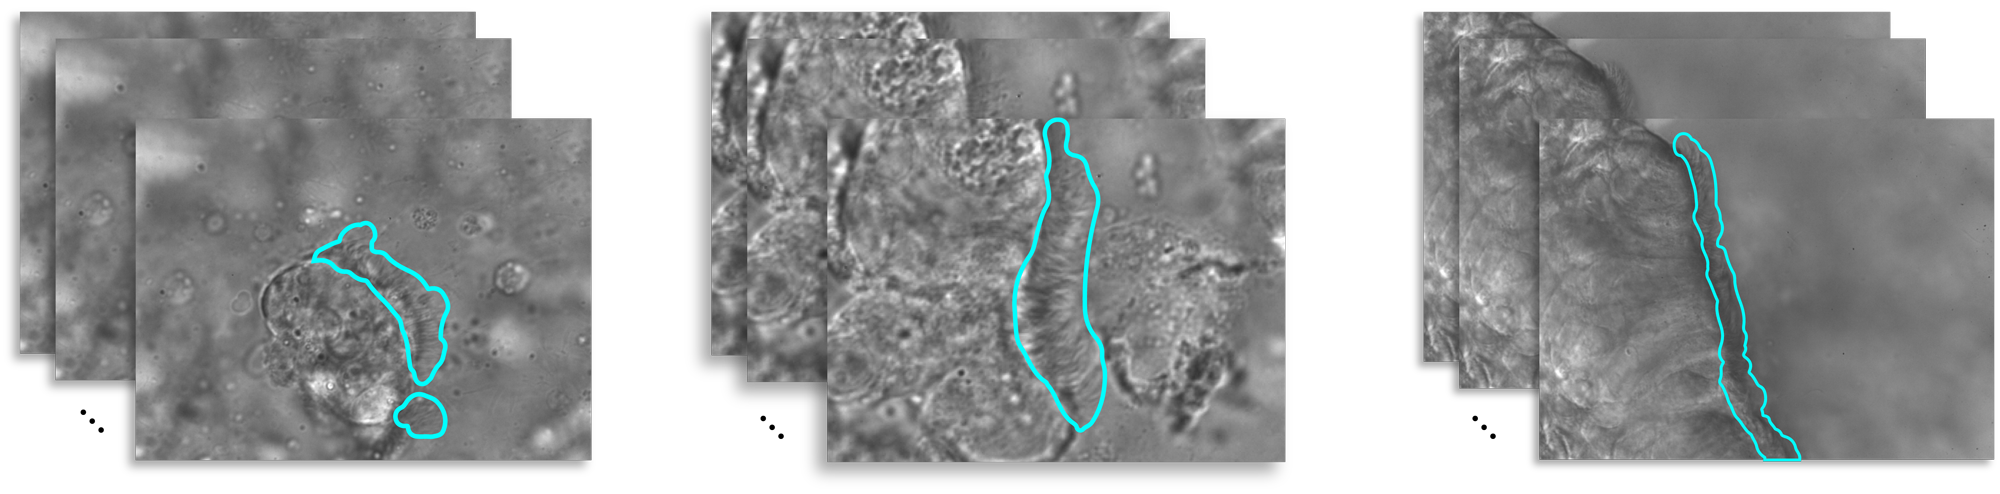
\includegraphics[width=.8\textwidth]{figures/cilia/sample_vids_with_gt_mask.png}
	\caption{A sample of three videos in our cilia dataset with their manually annotated ground truth masks.}
	\label{fig:sampleVidWithMask}
\end{figure}



Figure ~\ref{fig:sampleVidWithMask} shows a sample of the OF component at a random time. From OF vectors, elemental components such as rotation are derived, which highlights the ciliary motion by capturing twisting and turning movements. To model the temporal evolution of these motion vectors, we employ an autoregressive (AR) model $[@doi:10.5244/C.21.76]$. This model captures the dynamics of the flow vectors over time, allowing us to understand how the motion evolves frame by frame. The AR model helps in decomposing the motion into a low-dimensional subspace, which simplifies the complex ciliary motion into more manageable analyses.


\begin{equation}
	y_t =C\vec{x_t} + \vec{u}
	\label{eq:eq2}
\end{equation}

\begin{equation}
	\vec{x}_t = A_1\vec{x}_{t-1} + A_2\vec{x}_{t-2} + ... + A_d\vec{x}_{t-d} + \vec{v_t}
	\label{eq:eq3}
\end{equation}

In equation \eqref{eq:eq2}, $y_t$ represents the appearance of cilia at time t influenced by noise u. Equation \eqref{eq:eq3} represents the state x of the ciliary motion in a low-dimensional subspace defined by an orthogonal basis $C$ at time $t$, plus a noise term $v_t$ and how the state changes from $t$ to $t+1$.

Equation \eqref{eq:eq3} is a decomposition of each frame of a ciliary motion video yt into a low-dimensional state vector $x_t$ using an orthogonal basis $C$. This equation at position $x_t$ is a function of the sum of $d$ of its previous positions $ x_{t-1}, x_{t-2}, x_{t-d} $ each multiplied by its corresponding coefficients $A = A_1, A_2,..., A_d $. The noise terms $u$ and $v$ are used to represent the residual difference between the observed data and the solutions to the linear equations. The variance in the data is predominantly captured by a few dimensions of $C$, simplifying the complex motion into manageable analyses.

\begin{figure}[h]
	\centering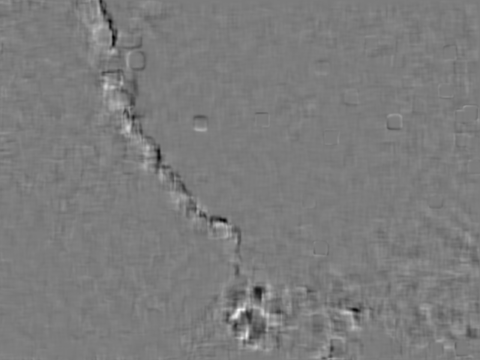
\includegraphics[width=0.5\textwidth]{figures/cilia/sample_OF.png}
	\caption{Representation of rotation (curl) component of OF at a random time.}
	\label{fig:sampleOF}
\end{figure}


Each order of the autoregressive model roughly aligns with different frequencies within the data, therefore, in our experiments, we chose d=5 as the order of our autoregressive model. This choice allows us to capture a broader temporal context, providing a more comprehensive understanding of the system’s dynamics. We then created raw masks from this lower-dimensional subspace, and further enhanced them with adaptive thresholding to remove the remaining noise.





In ~\ref{fig:sampleOF} , the first-order AR parameter is showing the most variance in the video, which corresponds to the frequency of motion that cilia exhibit. The remaining orders have correspondence with other different frequencies in the data caused by, for instance, camera shaking. Evidently, simply thresholding the first-order AR parameter is adequate to produce an accurate mask, however, in order to get a more refined result we subtracted the second order from the first one, followed by a Min-Max normalization of pixel intensities and scaling to an 8-bit unsigned integer range. We used adaptive thresholding to extract the mask on all videos of our dataset. The generated masks exhibited under-segmentation in the ciliary region, and sparse over-segmentation in other regions of the image. To overcome this, we adapted a Gaussian blur filter followed by an Otsu thresholding to restore the under-segmentation and remove the sparse over-segmentation. Figure ~\ref{fig:thresholding} illustrates the steps of the process.

\begin{figure}[h]
	\centering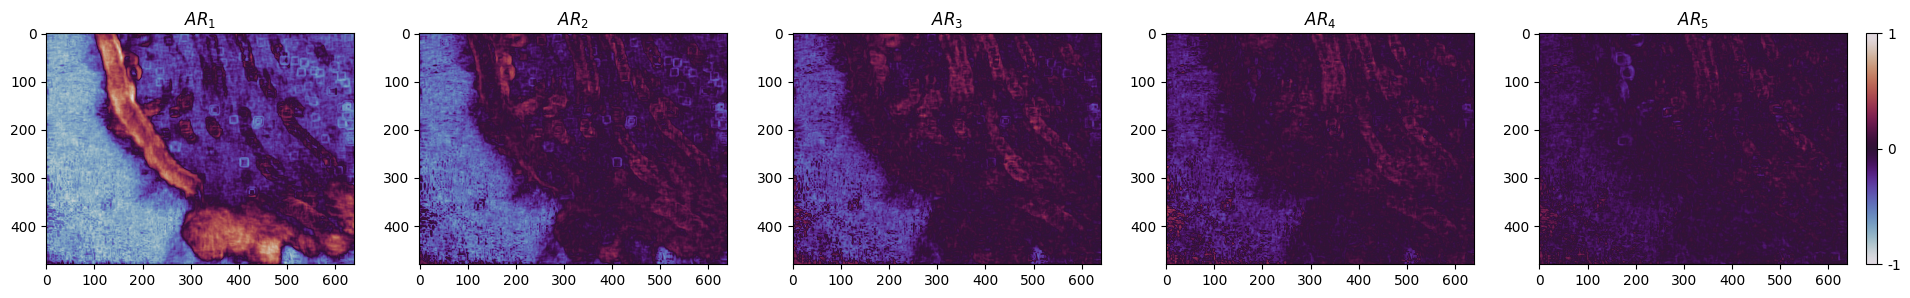
\includegraphics[width=1\textwidth]{figures/cilia/AR matrices.png}
	\caption{The pixel representation of the 5-order AR model of the OF component of a sample video. The x and y axes correspond to the width and height of the video.}
	\label{fig:ARMatrices}
\end{figure}


\begin{figure}[h]
	\centering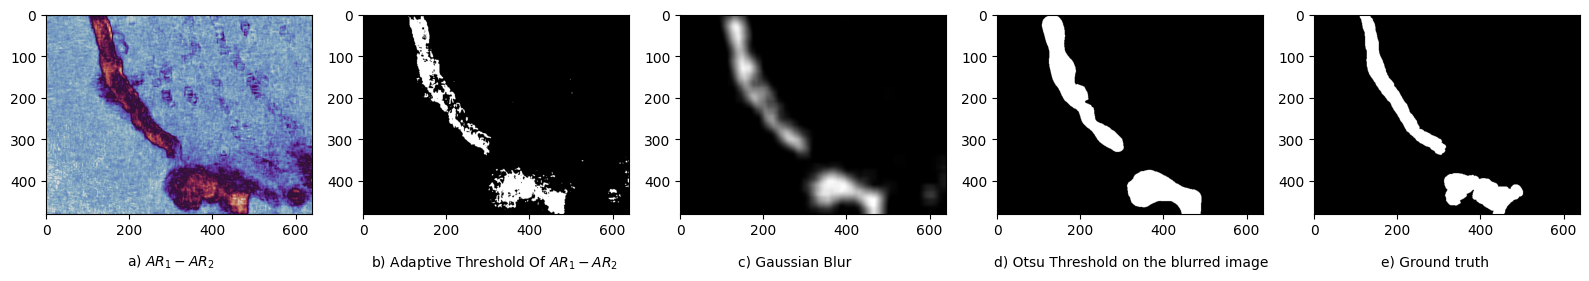
\includegraphics[width=1\textwidth]{figures/cilia/thresholding.png}
	\caption{The process of computing the masks. \textbf{a)} Subtracting the second-order AR parameter from the first-order, followed by \textbf{b)} Adaptive thresholding, which suffers from under/over-segmentation. \textbf{c)} A Gaussian blur filter, followed by \textbf{d)} An Otsu thresholding eliminates the under/over-segmentation.}
	\label{fig:thresholding}
\end{figure}

\section{Training the model}
Our dataset includes 512 videos, with 437 videos of dyskinetic cilia and 75 videos of healthy motile cilia, referred to as the control group. The control group is split into \%85 and \%15 for training and validation respectively. 108 videos in the dyskinetic group are manually annotated which are used in the testing step. Figure ~\ref{fig:sampleVidWithMask} shows annotated samples of our dataset.
\begin{figure}[h]
	\centering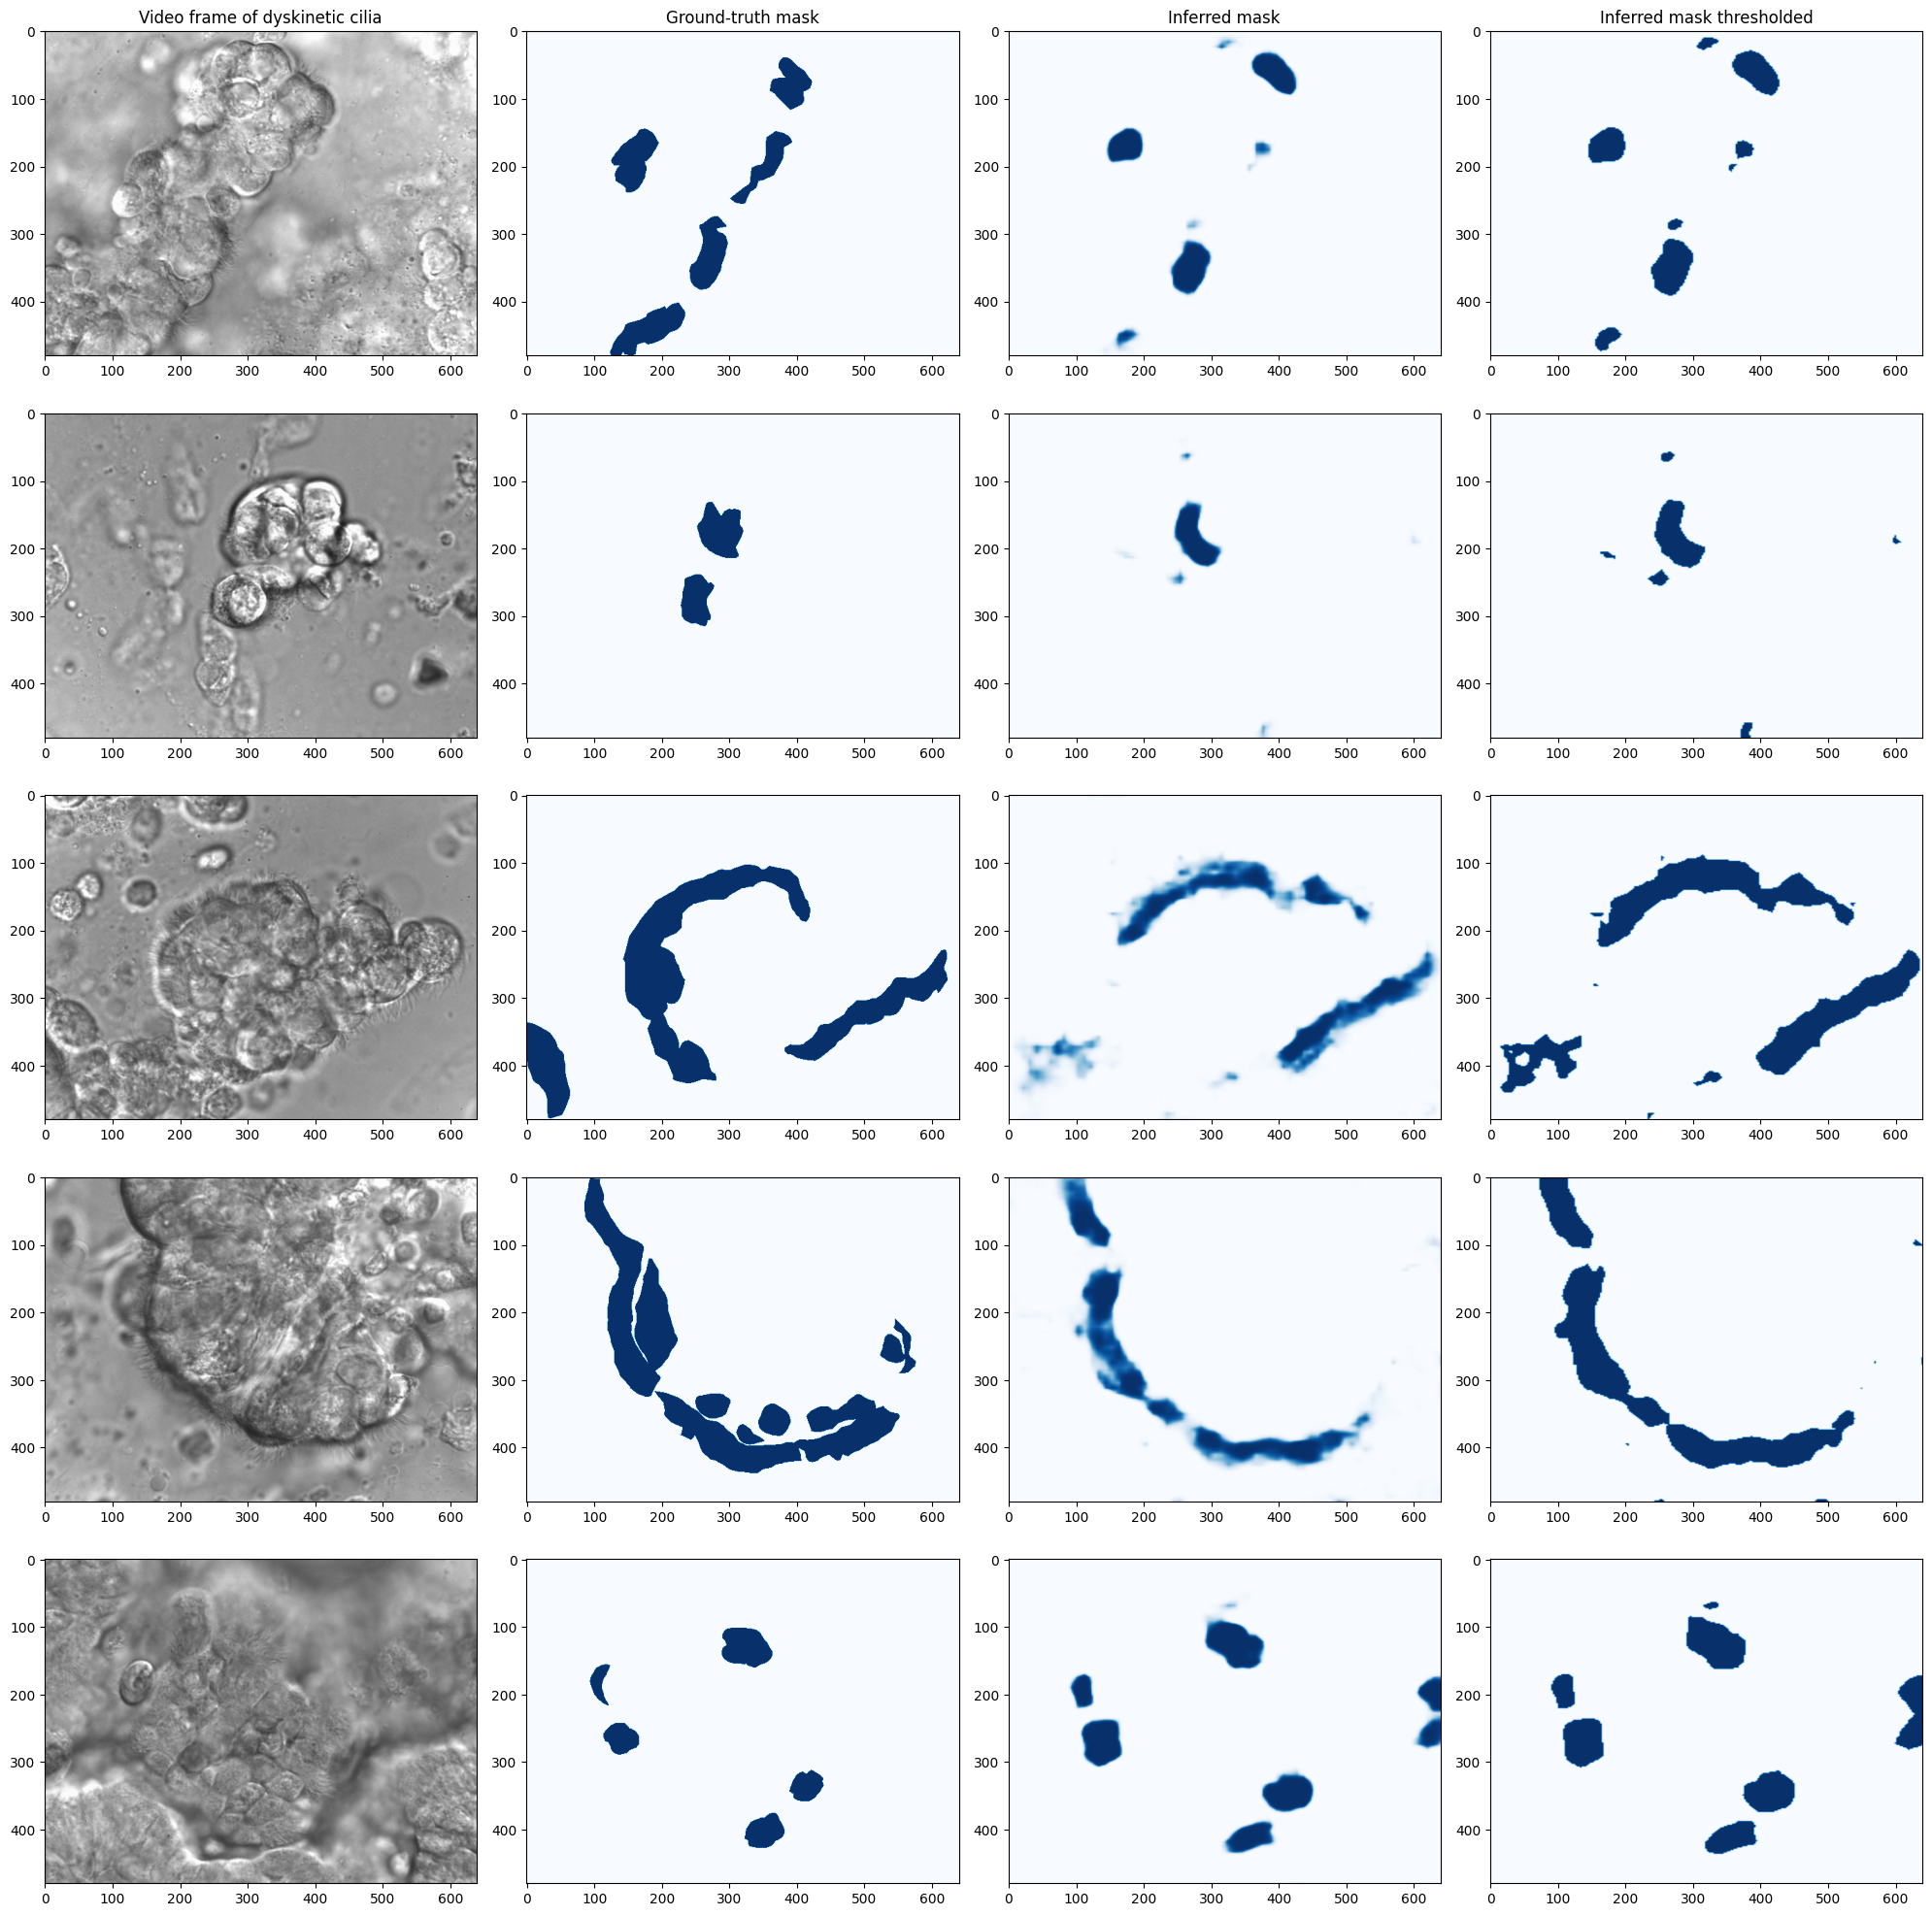
\includegraphics[width=.6\textwidth]{figures/cilia/out_sample.png}
	\caption{The model predictions on 5 dyskinetic cilia samples. The first column shows a frame of the video, the second column shows the manually labeled ground truth, the third column is the model’s prediction, and the last column is a thresholded version of the prediction.}
	\label{fig:outSample}
\end{figure}

In our study, we employed a Feature Pyramid Network (FPN) $[@kirillov2017unified]$ architecture with a ResNet-34 encoder. The model was configured to handle grayscale images with a single input channel and produce binary segmentation masks. For the training input, one mask is generated per video using our methodology, and we use the first 250 frames from each video in the control group making a total of 18,750 input images. We utilized Binary Cross-Entropy Loss for training and the Adam optimizer with a learning rate of $10^{-3}$. To evaluate the model’s performance, we calculated the Dice score during training and validation. Data augmentation techniques, including resizing, random cropping, and rotation, were applied to enhance the model’s generalization capability. The implementation was done using a library $[@Iakubovskii:2019]$ based on PyTorch Lightning to facilitate efficient training and evaluation. Table \ref{tbl:model_specs} contains a summary of the model parameters and specifications.
\begin{table}[ht]
	\centering
	\caption{Summary of model architecture, training setup, and dataset distribution}
	\label{tbl:model_specs}
	\renewcommand{\arraystretch}{1.3} % Adjust row spacing
	\begin{tabular}{|l|p{10cm}|}
		\hline
		\textbf{Aspect}              & \textbf{Details}                                                                                         \\ \hline
		Architecture                 & FPN with ResNet-34 encoder                                                                               \\ \hline
		Input                        & Grayscale images with a single input channel                                                             \\ \hline
		Number of Epochs             & 20                                                                                                       \\ \hline
		Batch Size                   & 4                                                                                                        \\ \hline
		Training Samples             & 15,662                                                                                                   \\ \hline
		Validation Samples           & 2,763                                                                                                    \\ \hline
		Test Samples                 & 108                                                                                                      \\ \hline
		Loss Function                & Binary Cross-Entropy Loss                                                                                \\ \hline
		Optimizer                    & Adam optimizer with a learning rate of $10^{-3}$                                                         \\ \hline
		Evaluation Metric            & Dice score during training and validation                                                                \\ \hline
		Data Augmentation Techniques & Resizing, random cropping, and rotation                                                                  \\ \hline
		Implementation               & Using a Python library with Neural Networks for Image Segmentation based on PyTorch ${Iakubovskii:2019}$ \\ \hline
	\end{tabular}
\end{table}
% The next section discusses the results of the experiment and the performance of the model in detail.



\section{Results and Discussion}
The model’s performance metrics, including IoU, Dice score, sensitivity, and specificity, are summarized in @tbl:metrics. The validation phase achieved an IoU of 0.312 and a Dice score of 0.476, which indicates a moderate overlap between the predicted and ground truth masks. The high sensitivity (0.999) observed during validation suggests that the model is proficient in identifying ciliary regions, albeit with a specificity of 0.813, indicating some degree of false positives. In the testing phase, the IoU and Dice scores decreased to 0.230 and 0.374, respectively, reflecting the challenges posed by the dyskinetic cilia data, which were not included in the training or validation sets. Despite this, the model maintained a reasonable sensitivity of 0.631 and specificity of 0.787.




Figure ~\ref{fig:outSample} provides visual examples of the model’s predictions on dyskinetic cilia samples, alongside the manually labeled ground truth and thresholded predictions. The dyskinetic samples were not used in the training or validation phases. These predictions were generated after only 20 epochs of training with a small training data. The visual comparison reveals that, while the model captures the general structure of ciliary regions, there are instances of under-segmentation and over-segmentation, which are more pronounced in the dyskinetic samples. This observation is consistent with the quantitative metrics, suggesting that further refinement of the pseudolabel generation process or model architecture could enhance segmentation accuracy.


\begin{table}[ht]
	\centering
	\caption{The performance of the model in validation and testing phases.}
	\label{tbl:metrics}
	\renewcommand{\arraystretch}{1.3} % Adjust row spacing for better readability
	\begin{tabular}{|l|c|c|c|c|}
		\hline
		\textbf{Phases} & \textbf{IoU over dataset} & \textbf{Dice Score} & \textbf{Sensitivity} & \textbf{Specificity} \\ \hline
		Validation      & 0.312                     & 0.476               & 0.999                & 0.813                \\ \hline
		Testing         & 0.230                     & 0.374               & 0.631                & 0.787                \\ \hline
	\end{tabular}
\end{table}


These results show the potential of our approach to reduce the reliance on manually labeled data for cilia segmentation. The use of this unsupervised learning framework allows the model to generalize from the motile cilia domain to the more variable dyskinetic cilia, although with some limitations in accuracy. Future work could focus on expanding the dataset and improving the process of generating pseudolabels to enhance the model’s accuracy.


\section{Conclusions and Final Remarks}
In this study, we introduced a self-supervised framework for cilia segmentation that eliminates the need for expert-labeled ground truth segmentation masks. Our approach takes advantage of the inherent visual similarities between healthy and unhealthy cilia to generate pseudolabels from optical flow-based motion segmentation of motile cilia. These pseudolabels are then used as ground truth for training a semi-supervised neural network capable of identifying regions containing dyskinetic cilia. Our results indicate that the self-supervised framework is a promising step towards automated cilia analysis. The model’s ability to generalize from motile to dyskinetic cilia demonstrates its potential applicability in clinical settings. Although there are areas for improvement, such as enhancing segmentation accuracy and expanding the dataset, the framework sets the foundation for more efficient and reliable cilia analysis pipelines.









% Dissertations will most likely include numerous side comments that are tangential to the main text. Generally, these are included in the document as footnotes or endnotes. With this template, you have the option to include them as \textit{sidenotes}, meaning they appear in the margin of your page rather than at the bottom.\footnote{Prior to 2020, this layout had not been used in a UGA dissertation. However, because of this {\LaTeX} template, the Graduate School and the format checkers approved the use of sidenotes specifically for us!} In this ``chapter'', we'll\footnote{I'll mention that this chapter was written primarily by Joey Stanley, so you'll know who's talking when I express my typographical opinions.} weigh the benefits and drawbacks of sidenotes and show you how you can toggle between them in your document.

%     \section{Turning sidenotes on}

%     The way to turn sidenotes on in this template is pretty straightforward. In the \texttt{dissertation.tex} file, you should find a command called \verb+sidenotetrue+. All you need to do is delete that line of code and type \verb+sidenotefalse+.

%     \section{List of changes}

%     If you do choose to turn the sidenotes on, be aware that it makes a couple other changes to your document. This section lists those changes.

%     \subsection{Changes to the footnote command}

%     The biggest change to your code is that the \verb+\footnote+ command has been recoded to now produce sidenotes. Specifically, the code that accomplishes this rewriting:
%     \begin{verbatim}
%       \renewcommand{\footnote}$[1]${
%           \sidenote{\RaggedRight\footnotesize #1}
%       }
%     \end{verbatim}
%     This code essentially turns the \verb+\footnote+ function into a wrapper around the \verb+\sidenote+ function from the \texttt{sidenote} package. It also changes the default fully-justified behavior to ``ragged right.''\footnote{With a sidenote margin so small, it's basically impossible to have good-looking text if it's forced to align to the left and right margins. Using \texttt{RaggedRight} from the \texttt{ragged2e} package does a nice job at making a narrow column of text look nice.} Finally, it ensures the font size is footnote size.

%     The reason for redefining \verb+\footnote+ rather than using \verb+\sidenote+ is becaue I wanted to make toggling between them as simple as possible. If you're three chapters into your dissertation and you decide you want to switch to the other layout, all you need to do is change one line of code. Had I required you to use \verb+\sidenote+, you would have to change the one command \textit{and} change all the \verb+\footnote+ commands to \verb+\sidenote+. I think doing it this way makes sense.

%     \subsection{Changes to the page layout}

%     If you have footnotes, the margins of your paper will be 1 inch on all sides, except for the bottom which is 1.25 inches.\footnote{This extra space is typo\-grahpically recommended to give the page a more balanced appearance.}. The body of the text is therefore centered, and there is no difference between even- and odd-sided pages.

%     If you turn on the sidenotes though, we needed to make some extra room to accomodate them in the margin.\footnote{Ideally, we'd make the paper wider so that it's slightly more square. Most books that use sidenotes today are like that. It gives a little extra width to the margins so the sidenotes aren't so narrow. Alas, we are constrained by UGA and Print \& Copy in Tate since they can only bind specific paper sizes.} To accomplish this, we had to reformat the layout on the page.

%     The biggest change is that the body of the text is now off-center. For odd-sided pages (meaning it would appear on the right side when you lay the book open), it's shifted towards the left and for even-sided pages (the left side of a two-page spread), it's shifted towards the right. In other words, the text is shifted towards the spine of the book. This leaves some room for the margins, which are towards the edges of the book. Here are the default dimensions:

%     \begin{itemize}
%       \item The top margin is 1 inch and the bottom margin is 1.25 inches.
%       \item Starting from the edge of the page (on an odd-sided page), the outer margin is 0.75 inches. This is the distance from the page to the edge of your sidenotes.
%       \item The sidenotes themselves are 1.5 inches wide.
%       \item There is a one-eighth inch space between the sidenotes and the body text.
%       \item The body text itself is 4.375 inches wide.
%       \item The inner margin is 1 inch.
%       \item There is an additional ``binding offset'' of a quarter inch added to the inside margin to accomodate for printing. This basically just means that the inside margin is 1.25 inches.
%     \end{itemize}
%     The outer margin has to be a little bit narrower than the typical 1 inch to give the body text enough room. Because footnotes are left-justified, this is not as noticeable on odd-sided pages, though on even-sided pages it's a little more obvious.



%     \section{Details about how sidenote behavior}

%     You should be aware of how the sidenotes behave, as they are implemented in this document. Sidenotes will be placed on the outer marin, but its their vertical positioning that may shift around.

%     By default, sidenotes will start on the same line as the sidenote \textit{marker} (that is, the small superscripted number within the body of your text). If you use relatively few sidenotes, or if they're generally short, this is what you'll typicaly find.

%     The question then is what happens if a sidenote runs up against the bottom of the page. Like if the sidenote marker is on the bottom line of a page and the sidenote itself is several lines long. As expected, the position of the sidenote itself will simply shift up so that it doens't spill into the bottom margin. Under the hood, while it is important that a sidenote be near its marker, is is \textit{more} important for the sidenote to not spill into the bottom margin, so that takes priority.

%     Similarly, if you have multiple sidenotes that are near each other, the notes themselves will not overlap. They'll reposition themselves vertically along the margin so that they're as close to their markers as possible without overlapping with eaach other or with a top/bottom margin.

%     For very long sidenotes,\footnote{Here is a very long sidenote so you can get a feel for what it looks like. Lorem ipsum dolor sit amet, consectetur adipisicing elit, sed do eiusmod tempor incididunt ut labore et dolore magna aliqua. Ut enim ad minim veniam, quis nostrud exercitation ullamco laboris nisi ut aliquip ex ea commodo consequat. Duis aute irure dolor in reprehenderit in voluptate velit esse cillum dolore eu fugiat nulla pariatur. Excepteur sint occaecat cupidatat non proident, sunt in culpa qui officia deserunt mollit anim id est laborum. Lorem ipsum dolor sit amet, consectetur adipisicing elit, sed do eiusmod tempor incididunt ut labore et dolore magna aliqua. Ut enim ad minim veniam, quis nostrud exercitation ullamco laboris nisi ut aliquip ex ea commodo consequat. Duis aute irure dolor in reprehenderit in voluptate velit esse cillum dolore eu fugiat nulla pariatur. Excepteur sint occaecat cupidatat non proident, sunt in culpa qui officia deserunt mollit anim id est laborum.} or for pages with many sidenotes such that they fill the margin completely, {\LaTeX} will do what it can to put it on the same page as the marker, but if it cannot, it will push it to the next page. For long footnotes, you may have seen them start on the correct page but spill over onto the next page---that behavior is unfortunately not possible with the current implementation of sidenotes in this template. For the most part this behavior is fine and readers typically are aware enough to look on the next page. However, be aware that should this next page be, say, the start of a new chapter, you'll get some unexpected sidenote placements.

%     For sidenotes that are so long that they cannot fit on a single page, it will cause an error in {\LaTeX} and your document will not compile. If you typically have many very long sidenotes, it may be better to switch to a footnote layout.



%     \section{Pros and Cons}

%     With this information in mind, it's important to consider the pros and cons of using sidenotes.

%     \subsection{Why I love sidenotes}

%     There are lots of reasons why I love sidenotes. First off, since they were popularized by statisticiaon Edward Tufte\footnote{Note that there is a \texttt{tufte} package that creates sidenotes. Because we did not necessarily want to use the other changes that package makes to the document, we chose not to use it here.} in his books on data visualization, they've been used widely and are adopted by many typographers. The reason is simple: they just look nice. Rather than your eye having to dart to the bottom of the page and back, sidenotes are \textit{in situ}, and they do a nice job at making it easier for the reader to find them.

%     In addition to making the sidenotes themselves easier to find and read, increasing the margin on one side makes the body text a little narrower. The typical 6.5 inch body text with 10- or 12-point font is a little too wide. The narrower layout, together with an appropriate line spacing, makes for a sophisticated layout that's easier to read than what you might be used to in a dissertation.

%     Sidenotes are nice for putting some kinds of additional, non-textual information that are very vertical. It's possible to put a very narrow table, a very narrow image, or even a smaller image,\footnote{There's no need for an image to take up half a page when the information can be conveyed in tiny plot. Here's an actual image I included in my dissertation, showing the distribution of a particular variable. \includegraphics$[width = 1.5in]${figures/tiny.pdf} It was handy to be able to have several of these little guys scattered around in the margins rather than taking up a huge chunk of the page.} icon, or plot in a sidenote.


%     \subsection{Why you may not love sidenotes}

%     First, as just mentioned, they're not ideal if you often use many long footnotes. If that's the case, you would probably be better off with the footnotes option.

%     Another small issue relates to how this particular template is structured. You can work on each chapter and compile each chapter individually. However, because the command that reorganizes the layout on the page is on the \texttt{dissertation.tex} file, when you compile just a single chapter, you don't get the right layout. This can be kind of annoying.

%     For certain things that may go in footnotes but are inherently wider, like formulas, computer code, extended quotations, data, numbered examples, or images, sidenotes are just too narrow. You're better off switching to footnotes if you make use of many of these. You may find a way to hack a one-off footnote if you need it for just one case.

%     Finally, because I've redefined \verb+\footnote+ to do sidenotes, it's not possible to include both footnotes and sidenotes within your document. I have seen some books do this, but I'm not sure why you would need both. Fortunately, this is an easy fix: you would just remove the code in \texttt{dissertation.tex} that redefines footnotes, and now you're free to use \verb+\footnote+ and \verb+\sidenote+ independently of each other. This behavior has not been tested so you're on your own as far as debugging goes.



%     \section{Hacking some less common cases}

%     \subsection{Putting a plot in a sidenote}

%     The code for the little plot I have in the sidenote above is this:
%     \begin{verbatim}
%       \includegraphics$[width = 1.5in]${figures/tiny.pdf}
%     \end{verbatim}
%     Note that because these are so small, there is no figure number assigned to them and there's no caption. Consequently, they will not appear in the ``List of Figures'' in your frontmatter if you have one.

%     \subsection{Others?}

%     TODO.

% \end{document}
